\documentclass[11pt]{article}
\usepackage{import}
\usepackage{hyperref,url}
\usepackage{amsmath,amssymb,amsthm}
\usepackage{tikz}
%\usepackage{float,subcaption,graphicx}
\usepackage{stmaryrd,wasysym,clrscode}
\usepackage{etex,etoolbox}
\usepackage{ifthen}
\usetikzlibrary{patterns,positioning}

%%% Added by Jonathan %%%
\def\[#1\]{\begin{align}#1\end{align}}
\def\(#1\){\begin{align*}#1\end{align*}}
\newcommand{\ip}[2]{\left\langle #1, #2 \right\rangle}
\definecolor{NAColor}{rgb}{.75,0,.75}
\newcommand{\NA}[1]{\textcolor{NAColor}{($\star$) #1}}
\newcommand{\dee}{\mathrm{d}}
\newcommand{\algname}[1]{\textsc{\lowercase{#1}}}
\def\argmax{\operatornamewithlimits{arg\,max}}
\def\argmin{\operatornamewithlimits{arg\,min}}
\newcommand{\defined}{\ensuremath{\triangleq}}
\newcommand{\bprf}{\begin{proof}}
\newcommand{\eprf}{\end{proof}}
\newcommand{\blem}{\begin{lemma}}
\newcommand{\elem}{\end{lemma}}
\newcommand{\eps}{\epsilon}
%%% End added by Jonathan %%%

\newcommand{\lc}[1]{#1_{\mathrm{loc}}}
\newcommand{\eq}[1]{\stackrel{\mathrm{#1}}{=}}
\DeclareMathOperator{\Var}{Var}
\DeclareMathOperator{\sign}{sign}
\DeclareMathOperator{\MMD}{MMD}
\newcommand{\MMDr}{\tilde{\MMD}}
\DeclareMathOperator{\Tr}{Tr}
\newcommand{\inner}[2]{\langle #1, #2 \rangle}
\newcommand{\E}{\mathcal{E}}
\newcommand{\eqdef}{\stackrel{\mathrm{def}}{=}}
\newcommand{\bP}{\mathbb{P}}
\newcommand{\bI}{\mathbb{I}}
\newcommand{\bE}{\mathbb{E}}
\newcommand{\sF}{\mathcal{F}}
\newcommand{\sH}{\mathcal{H}}
\newcommand{\sC}{\mathcal{C}}
\newcommand{\sM}{\mathcal{M}}
\newcommand{\sE}{\mathcal{E}}
\newcommand{\C}{\mathcal{C}}
\newcommand{\sB}{\mathcal{B}}
\newcommand{\bR}{\mathbb{R}}
\newcommand{\bN}{\mathbb{N}}
\newcommand{\bZ}{\mathbb{Z}}
\newcommand{\sI}{\mathcal{I}}
\newcommand{\sP}{\mathcal{P}}
\newcommand{\sX}{\mathcal{X}}
\newcommand{\sS}{\mathcal{S}}
\newcommand{\sJ}{\mathcal{J}}
\newcommand{\sR}{\mathcal{R}}
\newcommand{\sN}{\mathcal{N}}
\newcommand{\meet}{\wedge}
\newcommand{\RE}[2]{\operatorname{RE}\left(#1 \ \| \ #2\right)}
\newcommand{\KL}[2]{\operatorname{KL}\left(#1 \ \| \ #2\right)}
\newcommand{\KLm}[2]{\operatorname{KL}_m\left(#1 \ \| \ #2\right)}
\newcommand{\score}[2]{\operatorname{score}\left(#1 \ \| \ #2\right)}
\newcommand{\phih}{\hat{\phi}}
\newcommand{\psih}{\hat{\psi}}
\DeclareMathOperator{\supp}{supp}
\DeclareMathOperator{\loc}{loc}
\DeclareMathOperator{\lub}{lub}
\newcommand{\atom}[1]{#1^{\circ}}
\newcommand{\stitch}[2]{\overline{#1}^{#2}}
%\DeclareMathOperator{\argmin}{argmin}
%\DeclareMathOperator{\argmax}{argmax}

\newtheorem{theorem}{Theorem}[section]
\newtheorem{lemma}[theorem]{Lemma}
\newtheorem{proposition}[theorem]{Proposition}
\newtheorem{corollary}[theorem]{Corollary}
\newtheorem{assumption}[theorem]{Assumption}
\theoremstyle{definition}
\newtheorem{example}[theorem]{Example}
\newtheorem{definition}[theorem]{Definition}
\newtheorem{remark}[theorem]{Remark}
\newtheorem{property}[theorem]{Property}

\def\ci{\perp\!\!\!\perp}

\DeclareMathOperator{\Regret}{Regret}
\usepackage{fullpage}

\title{Exponentiated Gradient with Adaptive Regularization}
\author{Jacob Steinhardt}
\begin{document}
\maketitle
\section{Introduction}
Standard online learning algorithms obtain regret bounds that depend on the 
norm of the gradients $z_t$; for instance, exponentiated gradient has a regret bound 
of the form
\[ \Regret \leq \frac{\log(n)}{\eta} + \eta \sum_{t=1}^T \|z_t\|_{\infty}^2. \]
By using an analysis based on local norms, we can improve this to a bound
that also depends on the learner $w_t$:
\[ \Regret \leq \frac{\log(n)}{\eta} + \eta \sum_{t=1}^T \sum_{i=1}^n w_{t,i} z_{t,i}^2. \]
In this paper, we present a variant on the exponentiated gradient that instead 
obtains a bound depending on the competitor $w$:
\[ \Regret(w) \leq \frac{\log(n)}{\eta} + \eta \sum_{t=1}^T \sum_{i=1}^n w_{i}z_{t,i}^2. \]
This bound yields improvements when a component $i$ of the gradient is 
very noisy but has mean (across time) equal to zero. In this case 
$w_{t,i}z_{t,i}^2$ may be large but we can set $w_i$ to zero and thus $w_iz_{t,i}^2$ 
will be zero. 

Our algorithm has close connections to the multiplicative weights update method, 
which is a variant of exponentiated gradient that is sometimes used in the theory 
community to achieve better asymptotic loss bounds. We present a slight variant 
of this algorithm together with a novel analysis based on 
\emph{adaptively regularized mirror descent}, which clarifies the connection between 
exponentiated gradient and multiplicative updates and also explains why 
multiplicative updates sometimes yield better performance 
(because of the adaptive nature of the regularizer, versus a fixed regularizer for exponentiated gradient).

\section{Summary of Algorithms}
In this paper we compare three similar algorithms: exponentiated gradient, 
multiplicative updated, and adaptive exponentiated gradient. They are presented 
in Table~\ref{fig:alg1} in the case that all weights are constrained to the 
simplex. We later generalize to the unconstrained case but present the constrained 
versions here in order to contrast the three algorithms.

\begin{table}
\begin{tabular}{|c|c|c|} \hline
        Algorithm & Update & Regret \\ \hline
        Exponentiated gradient & $w_{t+1,i} \propto w_{t,i}\exp(-\eta z_{t,i})$ & $\frac{\log(n)}{\eta} + \eta \sum_{t=1}^T \sum_{i=1}^n w_{t,i}z_{t,i}^2$ \\ \hline
        Multiplicative updates & $w_{t+1,i} \propto w_{t,i}(1-\eta z_{t,i})$ & $\frac{\log(n)}{\eta} + \eta \sum_{t=1}^T \sum_{i=1}^n w_{i}z_{t,i}^2$ \\ \hline
        Adaptive exponentiated gradient & $w_{t+1,i} \propto w_{t,i}\exp(-\eta z_{t,i} - \eta^2 z_{t,i}^2)$ & $\frac{\log(n)}{\eta} + \eta \sum_{t=1}^T \sum_{i=1}^n w_iz_{t,i}^2$ \\ \hline
\end{tabular}
\caption{Comparison of exponentiated gradient, multiplicative updates, and adaptive exponentiated gradient algorithms on the simplex.}
\label{fig:alg1}
\end{table}

Each algorithm works by maintaining a weight vector $w_t \in \Delta_n$ and 
performing updates of the form $w_{t+1, i} \propto w_{t,i} \cdot f(z_{t,i})$, 
for some function $f$. The three cases are:
\begin{enumerate}
        \item \textbf{Exponentiated gradient:} $w_{t+1, i} \propto w_{t,i} \exp(-\eta z_{t,i})$ ($f(z) = \exp(-\eta z)$)
        \item \textbf{Multiplicative updates:} $w_{t+1, i} \propto w_{t,i} (1-\eta z_{t,i})$ ($f(z) = 1-\eta z$)
        \item \textbf{Adaptive exponentiated gradient:} $w_{t+1, i} \propto w_{t,i} \exp(-\eta z_{t,i}-\eta^2 z_{t,i}^2)$ ($f(z) = \exp(-\eta z - \eta^2 z^2)$)
\end{enumerate}
The first of these achieves regret that depends on the learner ($w_{t,i}z_{t,i}^2$) while the last two achieve regret that depends on the expert ($w_iz_{t,i}^2$).
Note that adaptive exponentiated gradient will tend to downweight any experts with high variance.

\section{Simple Example}
Suppose that there are $N$ experts, such that one has loss $-\epsilon$ always and the others 
each have loss alternating between $1$ and $-1$. 
Figure~\ref{fig:simple} shows the performance of all three 
algorithms in this setting, for $\epsilon = 0.1$, $T = 1000$, and $\eta = \sqrt{\frac{\log(N)}{T}}$. Note that the 
total regret of exponentiated gradient is $58$ in contrast to a regret of $39$ for adaptive 
exponentiated gradient. This is because the adaptive algorithm downweights all the high-variance 
experts due to the $\eta^2z_{t,i}^2$ term in the update.

We can ask what happens in the opposite case: when the optimal expert is high-variance and all 
the rest are low variance (for instance, the first expert has loss alternating bewteen $1-\epsilon$ 
and $-1-\epsilon$ while the rest have loss $0$ always). In this case being adaptive hurts us because 
we downweight the high-variance strategy even though it is optimal. Our regret is $88$ in contrast 
to the regret of $58$ of exponentiated gradient. In general, we should expect to do well when the optimal 
expert has low variance and poorly when the optimal expert has high variance. This is reflected 
in the regret bounds given in Table~\ref{fig:alg1}.

\begin{figure}
        \begin{center}
                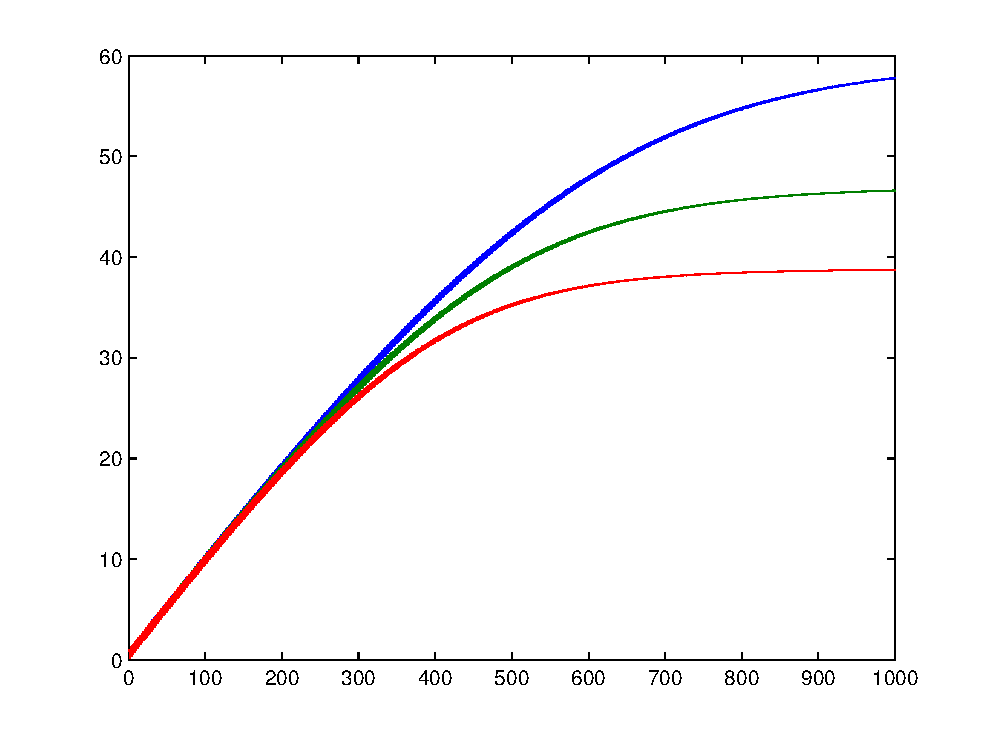
\includegraphics[width=0.4\textwidth]{simple.pdf} 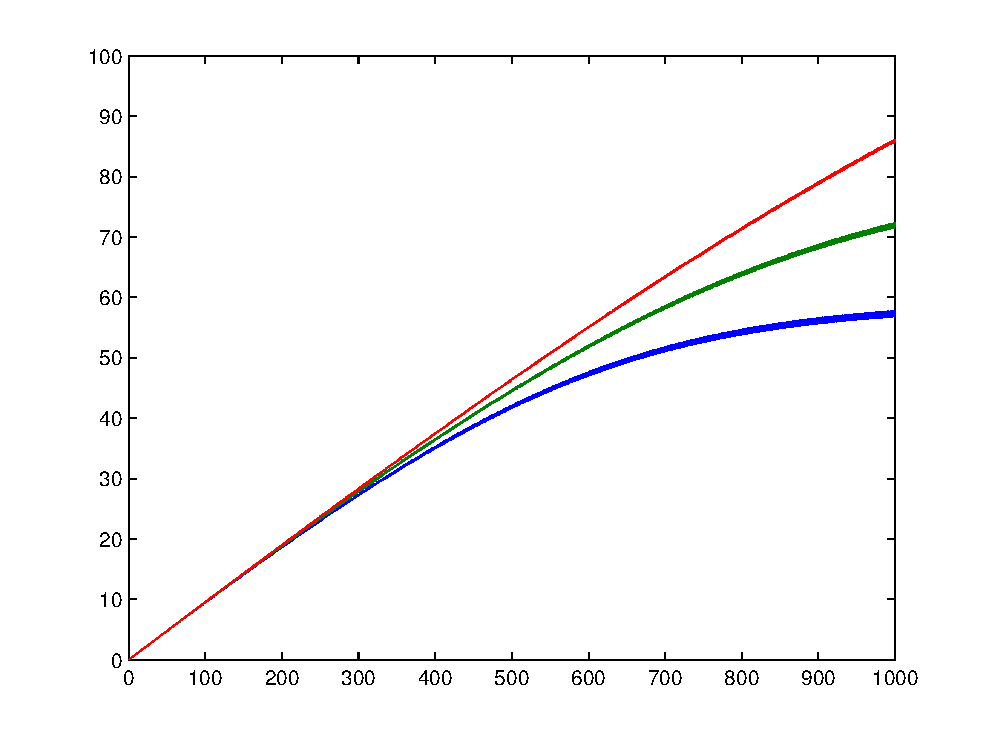
\includegraphics[width=0.4\textwidth]{tricky.pdf}
        \end{center}
        \caption{Regret as a function of time for exponentiated gradient (blue), multiplicative updates (green), and adaptive exponentiated gradient (red). Left: 
        the suboptimal strategies have high variance and the optimal strategy has low variance. Right: the suboptimal strategies have low variance and the 
        optimal strategy has high variance.}
        \label{fig:simple}
\end{figure}

\section{General Algorithms and Theoretical Analysis}
We now present the unconstrained versions of our three algorithms, together 
with an analysis based on adaptive regularizers. In each case, the weight 
vector $w$ is necessarily non-negative. We can deal with this constraint by 
maintaining two weight vectors $w_+$ and $w_-$ and predicting with $w_+-w_-$ 
(this is a standard idea, going back at least to the original exponentiated 
gradient paper by Kivinen and Warmuth). This is equivalent to replacing the 
gradient $z$ with the expanded vector $\left[ \begin{array}{cc} z \\ -z \end{array} \right]$. 
For simplicity of exposition, we will simply assume that $w$ is constrained 
to be non-negative in our algorithms and analysis.

Each algorithm can be interpreted as (adaptive) mirror descent with an appropriate 
regularizer. The regularizers are as follows:
\begin{enumerate}
        \item \textbf{Exponentiated gradient:} $\psi_t(w) = \sum_{i=1}^n w_i[\log(w_i/\lambda)-1]$.
        \item \textbf{Multiplicative updates:} $\psi_t(w) = \sum_{i=1}^n w_i[\log(w_i/\lambda)-1-\sum_{t=1}^T (\eta z_{t,i} + \log(1-\eta z_{t,i}))]$.
        \item \textbf{Adaptive exponentiated gradient:} $\psi_t(w) = \sum_{i=1}^n w_i[\log(w_i/\lambda)-1+\sum_{t=1}^T \eta^2 z_{t,i}^2 w_i]$.
\end{enumerate}
The parameter $\lambda$ is a hyperparameter controlling the size of $w$. Typically it should be on the order of $\frac{1}{n}$ 
(as we will see more explicitly when we prove a formal regret bound). Note that in the limit of small $\eta$, 
$-\eta z_{t,i} - \log(1-\eta z_{t,i}) \approx \frac{1}{2}\eta z_{t,i}^2$, so that 
the latter two regularizers are in fact very similar. The mirror descent updates corresponding 
to each of the above regularizers are:
\begin{enumerate}
        \item \textbf{Exponentiated gradient:} $w_{t,i} = \lambda \cdot \exp\left(-\eta \sum_{t=1}^T z_{t,i}\right)$
        \item \textbf{Multiplicative updates:} $w_{t,i} = \lambda \cdot \prod_{t=1}^T (1- \eta z_{t,i})$
        \item \textbf{Adaptive exponentiated gradient:} $w_{t,i} = \lambda \cdot \exp\left(- \sum_{t=1}^T \eta z_{t,i} + \eta^2 z_{t,i}^2\right)$
\end{enumerate}
Finally, we base our regret bounds on the following standard bound on the regret of mirror descent:
\begin{equation}
        \label{eqn:bound}
        \Regret(w) \leq \psi_T(w) + \sum_{t=1}^T D_{\psi_t^*}(\theta_{t+1} \| \theta_t).
\end{equation}
Our idea is to pick $\psi_{t+1}-\psi_t$ to cancel out the Bregman divergence term. The intuition is 
that we are absorbing all of our loss into the regularizer, therefore giving us a bound that depends 
on $w$ rather than $w_t$. This strategy is non-standard, although has been used before, for instance in 
various papers by Francesco Orabona. Note that in all three cases, $\psi_t(w)$ differs from $\psi_0(w)$ 
only in a linear term, and hence $D_{\psi_t^*} \equiv D_{\psi_0^*}$, and in particular 
$D_{\psi_t^*}(\theta_{t+1} \| \theta_t) \leq \sum_{i=1}^n w_{t,i}z_{t,i}^2$ by analysis via a local norm.

%%% We are interested in the following learning problem: our experts 
%%% consist of vectors $w \in \sH$, where $\sH$ is some convex 
%%% set; similarly, our adversary can play any move $z_t$ with 
%%% $z_t \in \sA$. A typical example is $\sH$ is the $n$-dimensional 
%%% simplex and $\sA$ is the unit $l^{\infty}$ ball. Our end goal is 
%%% to obtain a regret bound of the following type:
%%% \[ \sum_{t=1}^T w_t^Tz_t \leq \frac{\lambda}{\epsilon} + \epsilon \sum_{t=1}^T |w|^T|z_t| + \sum_{t=1}^T w^Tz_t. \]
%%% If we let $\sigma = \sup_{w \in \sH, z \in \sA} |w|^T|z|$, then the regret is bounded by
%%% $\frac{\lambda}{\epsilon} + \epsilon \sigma T$, which is equal to $2\sqrt{\lambda \sigma T}$ for 
%%% $\epsilon = \sqrt{\frac{\lambda}{\sigma T}}$. This is the type of regret bound that is typical 
%%% in most online learning settings. However, our bound can lead to stronger results in some 
%%% situations, for instance if $\sA$ is very asymmetrical about the origin, in which case 
%%% $|w|^T|z_t|$ will tend to be close to $w^Tz_t$ and we get bound
%%% \[ \sum_{t=1}^T w_t^Tz_t \leq \frac{\lambda}{\epsilon} + (1+\epsilon)\sum_{t=1}^T w^Tz_t, \]
%%% which is potentially much better, for instance if there is an expert that achieves 
%%% very small loss.
%%% 
%%% We propose the following general style of algorithm for obtaining such 
%%% bounds. The key innovation is an auxiliary variable $x_t$ that lets us 
%%% relate $w_t^Tz_t$ and $w^Tz_t$. The updates are as follows:
%%% \begin{align*}
%%% x_{t+1} &= f(x_t, \eta z_t) \\
%%% w_{t+1} &= \argmax_{w \in \sH} w^Tx_{t+1} - \psi(w) \\
%%% \Phi_{t+1} &= w_{t+1}^Tx_{t+1} - \psi(w_{t+1})  \\ &= \psi^*(x_{t+1}).
%%% \end{align*}
%%% 
%%% To see why these updates are a good idea, we will make a ``physicist's approximation'' 
%%% and suppose that $f(x_t, \eta z_t) \approx x_t - \eta z_t$. Then we would have
%%% \[ x_{T+1} \approx x_1 - \eta \sum_{t=1}^T z_t \] and thus, by definition, 
%%% \[ \Phi_{T+1} \gtrsim w^Tx_1 - \psi(w) - \eta \sum_{t=1}^T w^Tz_t. \]
%%% On the other hand, 
%%% \begin{align*}
%%% \Phi_{t+1} &\approx \Phi_t + w_t^T(x_{t+1} - x_t) \\
%%%            &= \Phi_t - \eta w_t^T z_t,
%%% \end{align*}
%%% so we have 
%%% \[ \Phi_{T+1} \approx \Phi_1 - \eta \sum_{t=1}^T w_t^Tz_t. \]
%%% Combining this with the preceding bound on $\Phi_{T+1}$ yields
%%% $\Phi_1 - \eta \sum_{t=1}^T w_t^Tz_t \gtrsim w^Tx_1 - \psi(w) - \eta \sum_{t=1}^T w^Tz_t$, 
%%% or
%%% \[ \sum_{t=1}^T w_t^Tz_t \lesssim \frac{\Phi_1 + \psi(w) - w^Tx_1}{\eta} + \sum_{t=1}^T w^Tz_t, \]
%%% which gives us an even better regret bound than we had sought (the $\sum_{t=1}^T |w|^T|z_t|$ term 
%%% will show up when we track the errors made in each of the approximations).
%%% 
%%% \paragraph{Formal statement.} To turn these approximations into a rigorous bound, we will 
%%% need $f$ and $\psi$ to satisfy the following properties:
%%% \begin{itemize}
%%% \item Concavity of $\psi^* \circ f$: $\psi^*(f(x,\eta z)) \leq \psi^*(x) - \eta w_x^Tz$, where $w_x = \partial \psi^*(x)$.
%%% \item Smoothness of $f$: $w^T(x-\eta z - f(x,\eta z)) \leq \eta^2 \alpha |w|^T|z|$ for all $w$.
%%% \end{itemize}
%%% (For some intuition, any $f$ satisfying the two properties above 
%%% must satisfy $f(x,0) = x$ and $f(x,\eta z) = x-\eta z + O(\eta^2)$.)
%%% \begin{theorem}
%%% \label{thm:main}
%%% Suppose that $\psi^*$ and $f$ satisfy the two properties above. Then, 
%%% for $\eta = \frac{\epsilon}{\alpha}$, we have the bound
%%% \[ \sum_{t=1}^T w_t^Tz_t \leq \alpha \frac{\Phi_1 + \psi(w) - w^Tx_1}{\epsilon} + \epsilon \sum_{t=1}^T |w|^T|z_t| + \sum_{t=1}^T w^Tz_t. \]
%%% \end{theorem}
%%% \begin{proof}
%%% By the first condition, we have
%%% \begin{align*}
%%% \Phi^{t+1} &= \psi^*(x_{t+1}) \\
%%%  &= \psi^*(f(x_t, \eta z_t)) \\
%%%  &\leq \psi^*(x_t) - \eta \left(\frac{\partial \psi^*}{\partial x_t}\right)^T z_t \\
%%%  &= \Phi_t - \eta w_t^T z_t,
%%% \end{align*}
%%% which by induction implies that
%%% \[ \Phi_{T+1} \leq \Phi_1 - \eta \sum_{t=1}^T w_t^Tz_t. \]
%%% By the second condition, we have
%%% \begin{align*}
%%% w^Tx_{t+1} &= w^Tf(x, \eta z) \\
%%%  &\geq w^Tx_t - \eta w^Tz_t - \eta^2 \alpha |w|^T|z_t|,
%%% \end{align*}
%%% which by induction implies that
%%% \[ w^Tx_{T+1} \geq w^Tx_1 - \eta^2\alpha \sum_{t=1}^T |w|^T|z_t| - \eta \sum_{t=1}^T w^Tz_t. \]
%%% Combining this with the first inequality yields
%%% \begin{align*}
%%% \Phi_1 - \eta \sum_{t=1}^T w_t^Tz_t &\geq \Phi_{T+1} \\
%%%  &\geq w^Tx_{T+1} - \psi(w) \\
%%%  &\geq w^Tx_1 - \psi(w) - \eta^2\alpha \sum_{t=1}^T |w|^T|z_t| - \eta \sum_{t=1}^T w^Tz_t.
%%% \end{align*}
%%% Re-arranging yields
%%% \[ \sum_{t=1}^T w_t^Tz_t \leq \frac{\Phi_1 + \psi(w) - w^Tx_1}{\eta} + \eta\alpha \sum_{t=1}^T |w|^T|z_t| + \sum_{t=1}^T w^Tz_t, \]
%%% which gives the desired result.
%%% \end{proof}
%%% 
%%% \paragraph{Relationship to mirror descent.} Mirror descent can be cast in the same framework as above, 
%%% and corresponds to the exact additive update $x_{t+1} = x_t - \eta z_t$. Thus while our algorithm 
%%% makes sure that $\psi^*$ decreases at a rate of $w_t^Tz_t$ and then bounds the error between 
%%% $x_{t+1}$ and $x_t - \eta z_t$, in contrast mirror descent sets the error between $x_{t+1}$ and 
%%% $x_t - \eta z_t$ to zero, and then relies on the smoothness of $\psi^*$ to bound the error between 
%%% $\psi^*(x-\eta z)$ and $\psi^*(x) - \eta w_x^Tz$.
%%% \section{Examples}
%%% \paragraph{Multiplicative updates.} If we let $\sH$ be the simplex and $\sA$ be the 
%%% $l^{\infty}$ ball of radius $r$, then a standard algorithm for minimizing regret is the 
%%% \emph{multiplicative weights update method}. We recover this by letting $f(x,z) = x + \log(1-z)$ 
%%% and $\psi(w) = \sum_{i=1}^n w_i\log w_i$. Then $\psi^*(x) = \log\left(\sum_{i=1}^n \exp(x_i)\right)$, 
%%% and $w_{t+1,i} = \exp(x_{t+1,i})/\sum_{j=1}^n \exp(x_{t+1,j})$.
%%% \begin{align*}
%%% \psi^*(f(x,\eta z)) &= \log\left(\sum_{i=1}^n \exp(x_i + \log(1-\eta z_i))\right) \\
%%%  &= \log\left(\sum_{i=1}^n \exp(x_i)(1-\eta z_i)\right) \\
%%%  &= \log\left(\sum_{i=1}^n \exp(x_i) - \eta \sum_{i=1}^n \exp(x_i) z_i\right) \\
%%%  &\leq \log\left(\sum_{i=1}^n \exp(x_i)\right) - \eta \frac{\sum_{i=1}^n \exp(x_i) z_i}{\sum_{i=1}^n \exp(x_i)} \\
%%%  &= \psi^*(x) - \eta w^Tz,
%%% \end{align*}
%%% so condition 1 is satisfied.
%%% 
%%% Also, using the fact that $\log(1-\eta z_i) \geq -\eta z_i - \eta^2 z_i^2$, we have
%%% \begin{align*}
%%% w^T(x-\eta z - f(x, \eta z)) &= w^T(x-\eta z - (x + \log(1-\eta z))) \\
%%%  &\leq \eta^2 \sum_{i=1}^n w_iz_i^2 \\
%%%  &\leq \eta^2 r \sum_{i=1}^n |w_i||z_i|,
%%% \end{align*}
%%% where in the last step we used the fact that $|z_i| \leq r$. These updates 
%%% thus fulfill the conditions of Theorem~\ref{thm:main} for $\alpha$ equal to 
%%% $r$.
%%% 
%%% \paragraph{Sum of pointed convex sets.} Suppose that our hypothesis class 
%%% $\sH \subseteq \bR^n$ can be decomposed as $\sH = \sH_+ + \sH_-$, where $\sH_+$ consists 
%%% only of non-negative vectors and $\sH_-$ consists only of non-positive vectors. 
%%% We can translate this into a problem n $\bR^{2n}$, by letting $\sH' \eqdef \sH_+ \times (-\sH_-)$ 
%%% and $\sA' \eqdef \{(z, -z) \mid z \in \sA\}$. Then $(w')^T(z') = w^Tz$. Now 
%%% let $(w_+, w_-)$ be the decomposition of $w'$ into its two components. We will 
%%% define
%%% \[ \psi(w') = \left\{ \begin{array}{ccl} \sum_{i=1}^n \log((w_+)_i + (w_-)_i) & : & w' \in \sH \\ \infty & : & \mathrm{else}. \end{array} \right. \]
%%% Now let 
%%% \[ R \eqdef \sup\limits_{w_+ \in \sH_+, w_- \in \sH_-, z \in \sA}  |w_+^Tz| + |w_-^Tz|, \]
%%% and consider the update $x_{t+1} = x_t - \eta z'_t - 2\eta^2 R |z'_t|$. Then we have
%%% \begin{align*}
%%% \psi^*(x_{t+1}) &= \psi^*(x_t) - \eta (w'_t)^T(z'_t) - 2\eta^2R (w'_t)^T|z'_t| + D_{\psi^*}(x_{t+1} \| x_t) \\
%%%  &= \psi^*(x_t) - \eta (w'_t)^Tz_t - 2\eta^2R (w'_t)^T|z'_t| + \frac{1}{2}((w'_t)^T|x_{t+1}-x_t|)^2 \\
%%%  &= \psi^*(x_t) - \eta (w'_t)^Tz_t - 2\eta^2R (w'_t)^T|z'_t| + \frac{1}{2}(\eta (w'_t)^T|z'_t| + 2\eta^2R (w'_t)^T|z'_t|)^2 \\
%%%  &= \psi^*(x_t) - \eta (w'_t)^Tz_t
%%% \end{align*}
%%% as long as $2\eta R \leq 1$, or $\eta \leq \frac{1}{2R}$. Thus the first condition is 
%%% satisfied. Also, by construction we have 
%%% \[ w^T(x_t - \eta z_t - x_{t+1}) = 2\eta^2 R w^T|z'_t|, \]
%%% so that the second condition is satisfied for $\alpha = 2R$. Combining these, and 
%%% setting $x_1 = 0$, we obtain the bound
%%% \[ \sum_{t=1}^T w_t^Tz_t \leq \frac{2R[\psi(w) - \inf_{\tilde{w}} \psi(\tilde{w})]}{\epsilon} + \epsilon \sum_{t=1}^T (w_+ + w_-)^T|z_t| + \sum_{t=1}^T w^Tz_t. \]
%%% This is a quite general result, but suffers from the fact that $\psi(w)$ can grow very large. 
%%% Finding ways to deal with this would thus be very interesting.
%%% 
%%% \paragraph{Inflated $l^p$ norm.} By abuse of notation, let $\alpha$ denote the vector 
%%% whose coordinates are all equal to $\alpha$. Let $\sH = B_{\alpha}^p(\lambda)$, where 
%%% \[ B_{\alpha}^p(\lambda) \eqdef \{w \mid w \geq \alpha, \|w-\alpha\|_p \leq \lambda \}. \]
%%% Note that this is the positive $l^p$ ball of radius $\lambda$, translated by $\alpha$. 
%%% (We will show below that we can embed the unconstrained $l^p$ ball into $B_{\alpha}^p(\lambda)$ 
%%% at the cost of increasing the dimension by a factor of 2, implying that 
%%% $B_{\alpha}^p(\lambda)$ is a rich hypothesis class.) 
%%% 
%%% We will let $\psi(w) = \left\{ \begin{array}{ccl} \frac{1}{2(p-1)}\|w-\alpha\|_p^2 & : & w \geq \alpha \\ \infty & : & w \not\geq \alpha. \end{array} \right.$. 
%%% Then 
%%% \[ \psi^*(x) = \alpha \sum_{i=1}^n x_i + \frac{1}{2(q-1)}\|x_+\|_q^2, \]
%%% where $x_+$ is the positive part of $x$ and $\frac{1}{p} + \frac{1}{q} = 1$.
%%% 
%%% Now suppose we use the update $x_{t+1,i} = x_{t,i} - \eta z_{t,i} - 2\eta^2 \frac{\|z\|_q^2}{\|z\|_1} |z_{t,i}| / \alpha$. 
%%% Note that the Bregman divergence $D_{\psi^*}(x_{t+1} \| x_t)$ is bounded above by the Bregman divergence 
%%% of $\frac{1}{2(q-1)}\|x\|_q^2$ (since it can be obtained from $\psi^*$ by adding a convex function), 
%%% which is in turn bounded above by $\frac{1}{2}\|x_{t+1}-x_t\|_q^2$. Using these facts, together with the fact that 
%%% $w \geq \alpha$, we have
%%% \begin{align*}
%%% \psi^*(x_{t+1}) &\leq \psi^*(x_t) - \eta w_t^Tz_t - \frac{2\eta^2\|z\|_q^2}{\alpha \|z\|_1} w_t^T|z_t| + D_{\psi^*}(x_{t+1} \| x_t) \\
%%%  &\leq \psi^*(x_t) - \eta w_t^Tz_t - \frac{2\eta^2\|z\|_q^2}{\alpha \|z\|_1} w_t^T|z_t| + \frac{1}{2}\left\|\eta z_t + \frac{2\eta^2\|z\|_q^2}{\alpha \|z\|_1} |z_t|\right\|_q^2 \\
%%%  &\leq \psi^*(x_t) - \eta w_t^Tz_t - 2\eta^2 \|z\|_q^2 + \frac{1}{2} \left(\eta \|z_t\|_q + \frac{2\eta^2\|z_t\|_q^3}{\alpha \|z_t\|_1}\right)^2 \\
%%%  &\leq \psi^*(x_t) - \eta w_t^Tz_t - 2\eta^2 \|z\|_q^2 + \frac{1}{2} \left(\eta \|z_t\|_q + 2\eta^2 \|z_t\|_{q}^2 / \alpha\right)^2 \\
%%%  &\leq \psi^*(x_t) - \eta w_t^Tz_t
%%% \end{align*}
%%% as long as $2\eta \|z_t\|_q/\alpha \leq 1$, which holds as long as $\eta \leq \frac{\alpha}{2r_q}$. In addition, we have that
%%% \begin{align*}
%%% w^T(x_{t} - \eta z_t - x_{t+1}) &= -\frac{2\eta^2\|z_t\|_q^2}{\alpha\|z_t\|_1}w^T|z_t| \\
%%%  &\leq \eta^2 \frac{2\|z_t\|_q}{\alpha} |w|^T|z_t| \\
%%%  &\leq \eta^2 \frac{2r_q}{\alpha} |w|^T|z_t|.
%%% \end{align*}
%%% So, both conditions of Theorem~\ref{thm:main} are satisfied. 
%%% If we set $x_1 = 0$, then $\psi^*(x_1) = 0$ as well.
%%% Therefore, for $\eta = \frac{\epsilon \alpha}{2r_q}$, we obtain a regret bound of 
%%% \[ \frac{2r_q\psi(w)}{\epsilon \alpha} + \epsilon \sum_{t=1}^T |w|^T|z_t|. \]
%%% Note that the regret gets smaller as $\alpha$ grows larger. This might seem too good 
%%% to be true, until we notice the following: if $\alpha$ is very large, then all 
%%% vectors with a small value of $\|w-\alpha\|_p$ will point in approximately the same 
%%% direction, and thus get similar (multiplicative) values for the regret.
%%% \paragraph{Embedding the $l^p$ ball into $B_{\alpha}^p$.} We now show how to turn problems 
%%% involving the $l^p$ ball into problems involving $B_{\alpha}^p$. Given a vector 
%%% $w \in \bR^n$, we can create a vector $w' \in \bR^{2n}$ via the embedding 
%%% $w \mapsto \left[ \begin{array}{c} \alpha + \max(w, 0) \\ \alpha - \min(w,0) \end{array} \right]$. 
%%% This embedding satisfies the property that $\|w\|_p = \|w'-\alpha\|_p$. Also, $w^Tz = w'^T\left[ \begin{array}{c} z \\ -z \end{array} \right]$. 
%%% If we plug into the regret bound above, the only difference is that the value of $|w|^T|z_t|$ increases, yielding 
%%% a regret of
%%% \[ \frac{r_q \|w\|_p^2}{\epsilon \alpha (p-1)} + \epsilon \sum_{t=1}^T \left(|w|^T|z_t| + 2\alpha \|z_t\|_1\right). \]
%%% Unfortunately, this final bound is quite bad, because the $\|z_t\|_1$ term grows with $T$ and depends on the 
%%% $l^1$ norm, which is the biggest of all the $l^p$ norms.
\end{document}
